\documentclass{report}
\usepackage[margin=0.7in]{geometry}

\usepackage{xcolor}
\usepackage{amsmath}
\usepackage{amsthm}
\usepackage{amssymb}
\usepackage{listings}
\usepackage{lipsum}
\usepackage{graphicx}

\title{STAT1301 - Lecture Notes}
\author{Ismael Khan}
\date{}

%\pagecolor{black}
%\color{white}


\theoremstyle{definition}
\newtheorem{definition}{Definition}
\newtheorem{example}{Example}

\theoremstyle{plain}
\newtheorem{theorem}{Theorem}
\newtheorem{lemma}{Lemma}
\newtheorem{cor}{Corollary}
\newtheorem{prop}{Proposition}
\newtheorem{conj}{Conjecture}

\theoremstyle{remark}
\newtheorem*{remark}{Remark}
\newtheorem*{note}{Note}
\newtheorem{case}{Case}

\begin{document}
\maketitle
\noindent
\chapter{Statistics Stuff}
\section{Lecture 5}
$$ \bar{x} = \frac{x_1 + x_2 + x_3 + ... + x_n}{n} = \frac{\displaystyle \sum_{i=1}^n x_i}{n} $$
The value $ b = \bar{x} $ minimizes the squared deviations from the data:
$$ \sum_{i=1}^n (x_i - b)^2 $$
\textbf{Prove this}
Observe that 
$$ g(b) = (170 - b)^2 + (182 - b)^2 + (160 - b)^2 $$
$$ g(b) = 3b^2 - \beta b - \gamma b -  $$
We can take the derivative to find the minimum
\begin{align*}
	g(b) &= \sum_{i=1}^n (x_i - b)^2\\
	g'(b) &= \sum_{i=1}^n 2(x_i -b) \cdot -1 = 0\\
	      &= test
\end{align*}

\subsection{Robustness}
What would happen if the third student had given their value in metres? Outliers can have a big effect on the sample mean. The median is also more informative for skewed data. Thus visualising is important before using means.

\subsection{Sample Variance}
Consider the three height values again: 170cm, 185cm, 162cm. How do we measure
the spread of these values?\\\\
One way to measure spread is via the sample variance:
$$ \beta = \frac{\sum_{i=1}^n (x_i - \bar{x})^2}{n-1} $$

\subsection{Sample standard deviation}
Note that the sample variance is on the squared scale of the original observations. To get a measure of spread on the original scale, we use the function
$$ \sigma = \sqrt{ \frac{\sum_{i=1}^n (x_i - \bar{x})^2}{n-1}} $$

Take an average height of people to be 170cm. A person of height 182cm leaves the room. The mean height will decrease. We can show this.
$$ \frac{x_1 + x_2 + x_3 + ... + x_n}{n} = 170 $$ Without loss of generality, that $ x_1 = 180 $, then $$ \frac{x_2 + ... + x_n}{n} = \frac{x_1 + x_2 + ... + x_n - x_1}{n-1}$$
$$ \frac{n \times 170 - 180}{n-1} < \frac{n \times 170 - 170}{n-1} = \frac{170(n-1)}{n-1} = 170 $$
\subsection{Uniform random numbers}

\section{Lecture 6}
\subsection{Modelling Relationships}
We often model relationships as a tend in the mean response plus variability about that trend.
$$ \gamma (x) = g(x) + \varepsilon $$
For $ \gamma $ being the response, $ x $ being the explanation variable and $ \varepsilon  $being the random error
\subsection{Describing Relations}
How much would describe the relationship between the father and son?

\subsection{Pearson Correlation}
The Pearson correlation coefficient $ r $, measures the strength of a linear relationship. If the points in the scatter plot are $ (x_1, y_1) $, $ (x_2, y_2) $, $ (x_n, y_n) $ then
$$ r = \frac{1}{n-1} \sum_{i=1}^n \Big ( \frac{x_i - \bar{x}}{s_x}\Big) \Big ( \frac{y_i - \bar{y}}{s_y}\Big) $$
It  is important to remember that $ r $ is only appropriate for linear relationships between variables.
\subsection{Least-Squared Lines}
Once we have determined that a straight line relationship may be appropriate we can go ahead and fit a line of best fit to the data. For any given line $ b_0 + b_1x $, how to judge how well it fits the data? We can look at the sum of the squared prediction error (or sum of squared deviations) 
$$ \sum_{i=1}^n (y_i - [b_0 + b_1x_i])^2 $$ 
The line $ b_0 + b_1 x_1 $, that minimises this is called the least-squares line.
\section{Lecture 7}
Probably skipped this to eat food
\section{Lecture 8}
I don't know anymore. What is the purpose of life. Who even is Joe Mama.
\subsection{Simple Probability Models}
The simplest probability model is when the sample spaces is a finite collection
of outcomes, all being equally likely.
\begin{example}[Rolling a Die]
  Consider rolling a fair 6 sided die. What is $ \Omega $?,
  $$ \Omega = \{1,2,3,4,5,6\} $$
  Then what is the probability $ \mathbb{P} $. For a given $ A \subset \Omega
  $, we assign the probability $ \mathbb{P}(A) $ as 
  $$ \mathbb{P}(A) = \frac{|A|}{|\Omega|}, \; A \subset \Omega $$
  Thus for $ |\Omega| = 6 $,
  $$ \mathbb{P}(A) = \frac{|A|}{6}, \; A \subset \Omega $$
\end{example}
% Counting Problem Notes
Drawing balls from an urn. The Urn can be counted in 4 possible urn experiments
\begin{enumerate}
  \item Ordered, with replacement
    (Notes missing)
  \item Ordered, without replacement  
  \item Unordered, without replacement \\\\
    Consider a horse race with 8 horses. How many ways are there to gamble on
    placings (1st,2nd,3rd).

  \item Unordered, with replacement
\end{enumerate}
\begin{center}
\fbox{\begin{minipage}{20em}
 \begin{theorem}
   Let $ X \sim U[a,b]$. Then,
   \begin{enumerate}
     \item $ \mathbb{E}(X) = \displaystyle \frac{(a+b)}{2} $
     \item $ Var(X) = \displaystyle \frac{(b-a)^2}{12} $
   \end{enumerate}
 \end{theorem} 
\end{minipage}}
\end{center}

\section{Lecture 9 - Conditional Probability and Independence}
\subsection{Conditional Probability}
How do we update the probability of an event $ A $ when we know that some other
event $ B $ has occured? If we are given that $ B $ has occured, then
$ A $ will occur if and only if $ A \cap B $ occurs.
\par The relative chance of $ A $ occuring given $ B $ has occured is therefore
$ \displaystyle \frac{\mathbb{P}(A \cap B)}{\mathbb{P}} $. Which is the
\textit{conditional probability} of $ A $ given $ B $.
\begin{center}
  \fbox{ \begin{minipage}{6.5in} \begin{definition} 
    The \textbf{condtional probability} of $ A $ given $ B $ is defined as.
    $$ \mathbb{P}(A\mid B) = \frac{\mathbb{P}(A\cap B)}{\mathbb{P}(B)} $$
    \end{definition}
    \end{minipage}}
\end{center}
\begin{example}
Suppose we have rolled a fair six-sided die. What is the conditional
probability that we get a "4" given we know that we rolled an \textit{even
number}.
\end{example}
Intuition implies that the probability is $ \displaystyle \frac{1}{3} $. We can
formally show this however.
\\\\
Let $ B $ be getting an even number $ = \{2,4,6\} $ and
$ A $ to be getting a 4 $ = \{4\} $. We already know that $ \mathbb{P}(B)
= \frac{3}{6} $. Now $ A \cap B = \{4\} $, so that $ \mathbb{P}(A \cap B)
= \frac{1}{6} $. Thus,
$$ \mathbb{P}(A\mid B) = \frac{\mathbb{P}(A\cap B)}{\mathbb{P}(B)}
= \frac{\frac{1}{6}}{ \frac{3}{6}} = \frac{1}{3} $$
\subsection{Product Rule}
Rearranging the definition of the conditional probability gives us an
expression for the product rule.
$$ \mathbb{P}(A\cap B) = \mathbb{P}(B) \mathbb{P}(A\mid B) = \mathbb{P}(A)
\mathbb{P}(B\mid A)$$
More generally,
$$ \mathbb{P}(A_1 \cap \dots \cap A_n) = \mathbb{P}(A_1) \mathbb{P}(A_2 \mid
A_1) \mathbb{P}(A_3\mid A_1 \cap A_2) \dots \mathbb{P}(A_n\mid A_1 \cap \dots
\cap A_{n-1}) $$
The crucial usage of this is that in many cases conditional probabilities are
easy to figure out.
\begin{example}
We draw consecutively 3 balls rom an urn with 5 white and 5 black balls,
without putting them back. What is the probability that all drawn balls will be
black? Let $ A_i $ be the event that the $ i $-th ball is black. We wish to
find the probability of $ A_1 \cap A_2 \cap A_3 $ (also written as $ A_1 A_2
A_3 $), which by the product rule is 
$$ \mathbb{P}(A_1) \mathbb{P}(A_2 \mid A_1) \mathbb{P}(A_3 \mid A_1 \cap A_2)
= \frac{5}{10} \frac{4}{9} \frac{3}{8} \approx 0.083 $$
\end{example}
\subsection{Independence}
If the join probability of two events $ A $ and $ B $ happens to factorise into
the product of the two individual probabilities, i.e.
$$ \mathbb{P}(A \cap B) = \mathbb{P}(A) \mathbb{P}(B) $$
Then we say that the events $ A $ and $ B $ are independent. In other words,
knowledge of $ A $ gives no additional knowledge to $ B $ and vice versa. This
implies that 
$$ \mathbb{P}(A\mid B) = \mathbb{P}(A) $$ 
and 
$$ \mathbb{P}(B\mid A) = \mathbb{P}(B) $$

\begin{example}
  Example 3 is used however 3 balls are chosen \textbf{with} putting them back.
  So by independence,
  $$ \mathbb{P}(A_1) \mathbb{P}(A_2 \mid A_1) \mathbb{P}(A_3 \mid A_1 \cap A_2)
  = \frac{5}{10} \frac{5}{10} \frac{5}{10} \approx 0.125$$
\end{example}

\section{Lecture 10 - Random Variables}
A random variable canbe viewed as measurement of a random experiemnt that
becomes available \textbf{tommorow}. However all the thinking about the
measurements can be carried out \textbf{today}. We denote random variables with
capital letters $ X, X_1, X_2, Y, Z $ etc.
\begin{example}
Some random variables may be
\begin{enumerate}
  \item THe number of defective transistors out of 100 inspected ones.
  \item The number of bugs in a computer program
  \item The amount of r ain in a certain location in June.
  \item The amount of time needed for an operation.
\end{enumerate}

We distinguish between discrete and continuous random variables:
\begin{itemize}
  \item \textbf{Discrete} random variables can only take \textit{countably
    many} values.
  \item \textbf{Continuous} random variables can take a \textit{continuous
    range} of values, for example, any value on the positive real line
    $ \mathbb{R}_+ $.
\end{itemize}
\end{example}
\subsection{Probability distrubition}
Let $ X $ be a random variable. We would like to designate the probabilities of
events such as $ \{X = x\} $ and $ \{a \leq X \leq b \} $. If we can specify
all probabilities involving $ X $, we say that we have determined the
probability distrubution of $ X $. 
\par A way to specifiy the P.D is to give all probabilties of the form $ \{X
\leq X\} $.
\begin{center}
\fbox{\begin{minipage}{6.5in}
\begin{definition}
  The \textbf{cumulative distribution function} (cdf) of a random variable
  $ X $ is the funciton $ F $ defined by
  $$ F(x) = \mathbb{P}(X \leq x), \; x\in \mathbb{R} $$
\end{definition}
\end{minipage}}
\end{center}
\subsection{Cumulative distribution function (cdf)}
Note that any cdf is increasing (if $ x \leq y $ then $ F(x) \leq F(y) $ and
lies inbetween 0 and 1. We can use any function $ F $ with these properties to
specify the distrubution of a random variable X
%Include figure

\subsection{Probability mass function}
\begin{center}
\fbox{\begin{minipage}{6.5in}
\begin{definition}
  A random variable $ X $ is said to have a discrete distrubution if
  $ \mathbb{P}(X=x_i) > 0, \; i = 1,2 ... $ for some finite or countable set of
  values $ x_1, x_2 ... $ such that $ \displaystyle \sum_{i} \mathbb{P}(X= x_i)
  = 1$. The \textbf{probability mass function (pmf)} of $ X $ is the function
  $ f $ defined by $ f(x) = \mathbb{P}(X=x) $.
\end{definition}
\end{minipage}}
\end{center}
By the sum rule, if we know $ f(x) \; \forall x$ then we can calculate all
possible probabilties involving $ X $
$$ \mathbb{P} (X \in B) = \displaystyle \sum_{x \in B}^{} f(x)  $$
\begin{note}
  $ \{X \in B\} $ should be read as $ X $ is an elemnt of $ B $ 
\end{note}

\begin{center}
\fbox{\begin{minipage}{6.5in}
\begin{definition}
A random variable $ X $ with cdf $ F $ is said to have a continuous
distrubution if there exists a positive function $ f $ with total integral
$ I $ such that $ \forall a < b $
$$ \mathbb{P} (a < X \leq b) = F(b) - F(a) = \int_a^b  f(u) \; du$$
Function $ f $ is called the \textbf{probability distribution function (pdf)}
of $ X $
\end{definition}
\end{minipage}}
\end{center}
\subsection{Calculating probabilities}
Once we know the pdf, we can calculate any probability taht $ X $ lies in some
set $ B $ by means of integration
$$ \mathbb{P} (X \in B) = \int_B  f(x) \; dx $$
\subsection{Relationship between cdf and pdf}
Suppose $ f $ and $ F $ are the pdf and cdf of a continuous random variable
$ X $ respectively. Then $ F $ is an anti-derivative of $ f $
$$ F(x) = \mathbb{P} (X \leq x) = \int_{-\infty}^x  f(u) \; du $$
Conversely, $ f $ is the derivative of the cdf $ F $
$$ f(x) = \frac{d}{dx} F(x) = F'(x) $$

\subsection{Density}
In the continuous case, $ f(x) \neq \mathbb{P} (X = x) $ because the latter is
0 $ \forall x $. Instead we intepret $ f(x) $ as the density of the probability
  at distrubution $ x $, in the sense that for any small $ h $. 
  $$ \mathbb{P} (x \leq X \leq x+h)  = \int_x^{x+h}  f(u) \; du \approx h f(x) $$

\begin{note}
  $ \mathbb{P} (x \leq X \leq x + h) = \mathbb{P} (x < X \leq x+h) $ in this
  case.
\end{note}
\begin{example}
  Draw a random number $ X $ from the interval of real numbers $ [0,2] $, where
  each number is equally likely to be drawn. What are the pdf and cdf $ F $ of
  X
\end{example}
We have
\[ \mathbb{P} (X \leq x) = F(x) = 
  \begin{cases}
    0 &\text{ if $ x < 0 $ } \\
    \displaystyle \frac{x}{2} &\text{ if 0 $ \leq x \leq 2 $ } \\
    1 &\text{ if $ x > 2 $}
  \end{cases}\]
  By differentiating $ F $ we find 
  \[ f(x) = \begin{cases}
    \frac{1}{2} &\text{if $ 0 \leq x \leq 2 $}\\
    0 &\text{otherwise}
  \end{cases} \]
  Note that theis density is constant on the interval $ [0,2] $ and zero
  elsewhere. Reflecting the fact that each point in $ [0,2] $ are equally
  \textbf{equally likely to be drawn}.
  \subsection{Expectation (discrete case)}
  Although all probability info about a random variable is contained in its
  cdf or pmf/pdf, it is often useful to consider various numerical
  characteristics of a random variable.
  \begin{center}
  \fbox{\begin{minipage}{6.5in}
  \begin{definition}
  Let $ X $ be a \textit{discrete} random variable with pmf $ f $. The
  \textbf{expectation} (or expected value) of $ X $, denoted as
  $ \mathbb{E}(X) $ is defined as 
  $$ \mathbb{E}(X) = \displaystyle \sum_{x}^{} x \mathbb{P} (X=x)
  = \displaystyle \sum_{x}^{} xf(x) $$
  \end{definition}
  \end{minipage}}
  \end{center}
  The expectation is thus a "weighted average" of the values that $ X $ can
  take.
  \subsection{Expectation (continuous case)}
  \begin{center}
  \fbox{\begin{minipage}{6.5in}
  \begin{definition}
  Let $ X $ be a \textit{continuous} random variable with pdf $ f $, The
  \textbf{expectation} (or expected value) of $ X $, denoted $ \mathbb{E}X $,
  is defined as
  $$ \mathbb{E}(X) = \int_{-\infty}^{\infty}  xf(x) \; dx $$
  \end{definition}
  \end{minipage}}
  \end{center}
  \subsection{Expectation of a function of a random variable}
  If $ X $ is a random variable, then a function of $ X $ such as $ X^2 $ or
  $ \sin(X) $ is also a random variable.
  \begin{center}
  \fbox{\begin{minipage}{6.5in}
      \begin{theorem}[Expectation of a Function of a Random Variable]
  If $ X $ is discrete with pdf $ f $, then for any real values function $ g $
  $$ \mathbb{E}(g(X)) = \displaystyle \sum_{x}^{} g(x)f(x) $$
  Replace the integral with a sum for the discrete case
  $$ \mathbb{E}(g(X)) = \int_{-\infty}^{\infty}  g(x)f(x) \; dx $$
  \end{theorem}
  \end{minipage}}
  \end{center}
%Examplse???

\subsection{Linearity of expectation}
An important consequence of Theorem 2 is that the expectation is "linear".
\begin{center}
\fbox{\begin{minipage}{6.5in}
    \begin{theorem}
    For any real numbers $ a $ and $ b $, and functions $ g $ and $ h $.
    \begin{enumerate}
      \item $\mathbb{E}(aX +b) = a\mathbb{E}(X) + b $
      \item $\mathbb{E}(g(X) + h(X)) = \mathbb{E}(g(X)) + \mathbb{E}(h(X)) $
    \end{enumerate}
    \end{theorem}
\end{minipage}}
\end{center}
\begin{proof}[Proof of Theorem 3] 
  We show it for the discrete case. Suppose $ X $ has pmf $ f $. The first
  statement follows from
  $$ \mathbb{E}(aX+b) = \displaystyle \sum_{x}^{} (ax+b)f(x) = a \displaystyle
  \sum_{x}^{} xf(x) + b \displaystyle \sum_{x}^{} f(x) = a \mathbb{E}(X) + b $$
  Similarly, the second statement follows from
  $$ \mathbb{E}(g(X) + h(X)) = \displaystyle \sum_{x}^{} (g(x) + h(x))f(x)
  = \displaystyle \sum_{x}^{} h(x)f(x)$$
  $$ \mathbb{E}(g(X)) + \mathbb{E}(h(X)) $$
\end{proof}
  \subsection{Variance}
  Another useful characteristic of the distrubution of $ X $ is the variance of
  $ X $. This number is sometimes denoted as $ \sigma^2 $ and measures the
  \textit{spread} of the distrubution of $ X $.
  \begin{center}
  \fbox{\begin{minipage}{6.5in}
  \begin{definition}
    The \textbf{variance} of a random variable $ X $, denoted $ \text{Var}(X)
    $, is defined as 
    $$ \text{Var}(X) = \mathbb{E}(X - \mu)^2 $$
    where $ \mu = \mathbb{E}(X) $. The square root of the variance is called
    the \textbf{standard deviation}. The number $ \mathbb{E}X' $ is called the
    r-th \textbf{moment} of $ X $
  \end{definition}
  \end{minipage}}
  \end{center}
  \subsection{Properties of Variance}
  \begin{center}
  \fbox{\begin{minipage}{6.5in}
  \begin{theorem}
  For any random variable $ X $, the following properties hold for variance
  \begin{enumerate}
    \item $ \text{Var}(X) = \mathbb{E}X^2 - (\mathbb{E}X)^2 $
    \item $ \text{Var}(a+bX) = b^2\text{Var}(X) $
  \end{enumerate}
  \end{theorem}
  \end{minipage}}
  \end{center}

  \subsection{Valuable Conclusions}
  \begin{itemize}
    \item The probability distrubution of a random variable is completely
      specified by its cdf (cumulative distrubution function). For discrete
      random variables, it is more useful to specifiy distrubution with pmf
      (probability mass function). For continuous random variables, use pdf
      (probability density function)
    \item The expectation (expected value) of a random variable is the weighted
      average of the values that random variable can take. It measures the
      locality of the distrubution of a random variable.
    \item The variance is the expected squared distance from the random
      variable to its expected value. As a consequence, it is a measure of the
      spread of distrubution of a random variable.
  \end{itemize}
  \begin{note}
    The lecture 11 (scheduled on a Wednesday) was cancelled due to the Ekka
    holiday. So all lectures proceeding from this point are one less then their
    \textit{true} lecture number.
  \end{note}
  \newpage
  \section{Lecture 11 - Bernoulli and binomial distribution}
  \subsection{Discrete random variables}
  \textbf{Discrete} random variables have only a finite or countable number of
  different values. Probabilities are calculated by summing the probability
  mass function (pmf)
  \begin{figure}[h]
    \centering
    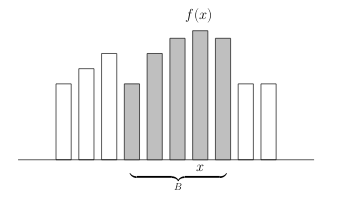
\includegraphics[width=0.6\linewidth]{1.png}
    \caption{Probability mass function (pmf)}%
    \label{fig:1}
  \end{figure}
  The most frequently used discrete probability distributions are the
  \textbf{Bernoulli} and \textbf{Binomial} distributions.

  \subsection{Bernoulli Trial}
  A \textbf{Bernoulli Trial} is a random experiment that has only two outcomes
  (success - 1, failure - 0). The random variable $ X $ is called the Bernoulli
  variable.
  \par An example may be a coin, two possible outcomes Heads or Tails, can be
  represented can be modelled as a Bernoulli variable attributing 1 for heads
  and 0 for tails.

  \begin{center}
  \fbox{\begin{minipage}{7in}
  \begin{definition}
  A random variable $ X $ is said to have a \textbf{Bernoulli} distribution
  with success probability $ p $ if $ X $ can only assume the values 1 and
  0 with probabilities 
  $$ \mathbb{P} (X = 1) = p \; \; \text{and} \; \; \mathbb{P} (X = 0) = 1 -p $$
  We write $ X \sim \text{Ber}(p) $
  \end{definition}
  \end{minipage}}
  \end{center}

  \begin{figure}[h]
    \centering
    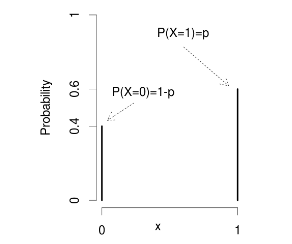
\includegraphics[width=0.6\linewidth]{2.png}
    \caption{Probability mass function for the Bernoulli distribution with
    parameter $ p $ (the case $ p = 0.6 $ is shown)}%
    \label{fig:2}
  \end{figure}

  \begin{center}
  \fbox{\begin{minipage}{7in}
  \begin{theorem}
    Let $ X \sim \text{Ber}(p) $. Then,
    \begin{enumerate}
      \item $ \mathbb{E}(X) = p $
      \item $ \text{Var}(X) = p(1-p) $
    \end{enumerate}
  \end{theorem}
  \end{minipage}}
  \end{center}
Lets prove this. \begin{proof}
  \begin{enumerate}
    \item \begin{align*}
  \mathbb{E}(X) &= \displaystyle \sum_{x}^{} xf(x) \\
		&= 0\cdot (1-p) + 1 \cdot p = p
\end{align*}
    \item \begin{align*}
	\text{Var}(X) &= \mathbb{E}(X-\mathbb{E}X)^2\\
	&= \mathbb{E}(X-p)^2 \\
	&= \mathbb{E}(X^2 - 2pX + p^2)\\
	&= \mathbb{E}X^2 + (\mathbb{E}(-2pX)) + \mathbb{E}p^2 \\
	&= \mathbb{E}X^2 - 2p\mathbb{E}X + p^2 \\ 
	&= \mathbb{E}X^2 - p^2 \\
	\intertext{Note that $ \mathbb{E}X^2 = 0^2(1-p) + 1^2\cdot p = p$}
	&= p - p^2 = p(1-p)
    \end{align*}
  \end{enumerate}
\end{proof}

\subsection{Counting possible outcomes}
If we observe the complete sequence of 100 tosses, there are $ 2^{100}
$ possible outcomes of the experiment, which are all equally likely (given
a fair coin).
\par To calculate the probability of having exactly $ x $ successes we need to
see how many of the possible outcomes have exactly $ x $ ones and $ 100
- x $ zeros. 
\\\\
There are $ \displaystyle {100 \choose x} $ of these, because we have to choose
exactly $ x $ positions for the 1s out of 100 possible positions.
We derive,
$$ \mathbb{P}(X=x) = \frac{\displaystyle {100\choose x}}{\displaystyle 2^{100}}
\;\; , x = 0,1,2, \dots, 100$$
This is an example of a Binomial distribution. We can now calculate
probabilities of interest such as $ \mathbb{P}(X \leq 60) $. We need to
evaluate
$$ \mathbb{P} (X \leq 60) = \displaystyle \sum_{x=60}^{100} \frac{\displaystyle
{100\choose x}}{2^{100}} = \frac{ \displaystyle \sum_{x=60}^{100} {100 \choose
x}}{2^{100}} $$
Which can be done in R with one line:
\begin{lstlisting}
> sum(choose)(100,60:100))/2^(100)

[1] 0.02844397
\end{lstlisting}

\subsection{Number of successes with a general coin}
Since the coin tosses are independent, we can use the product rule to find that
the probability of having a sequence of $ x $ heads and $ n-x $ tails is
$ p^x(1-p)^{n-x} $. However as there are still $ {n\choose x} $ of these
sequences. We can formalise this:

\begin{center}
\fbox{\begin{minipage}{7in}
\begin{definition}
A random variable $ X $ is said to have a \textbf{binomial} distribution with
parameters $ n $ and $ p $ if $ X $ can only assume the integer values of
$ x = 0,1,\dots,n $, with probabilities
$$ P(X=x) = {n\choose x} p^x (1-p)^{n-x}, \; \; x = 0,1,\dots,n $$
We write $ X \sim \text{Bin}(n,p) $
\end{definition}
\end{minipage}}
\end{center}


\paragraph{Tip:}
The number f successes in a series of $ n $ independent Bernoulli trials with
success probability $ p $ has a $ \text{Bin}(n,p) $ distribution

\begin{center}
\fbox{\begin{minipage}{7in}
\begin{theorem}
  Let $ X \sim \text{Bin}(n,p) $. Then,
  \begin{enumerate}
    \item $\mathbb{E}(X) = np$
    \item $ \text{Var}(X) = np(1-p) $
  \end{enumerate}
\end{theorem}
\end{minipage}}
\end{center}

\subsection{Binomial distribution in practice (cont.)}
Many practical statistical situations can be treated as a sequence of coin
flips. For example, we wish to conduct a survey of a large population to see
what proportion of $ p $ is male, where $ p $ is unknown.
\\\\
We can only know $ p $ if we observe everyone in the population, but we most
likely can't do that. So we select $ n $ people at random from the population
and record their gender. We assume that each person is chosen with equal
probability. 
\\\\
If we allow the same person to be selected more than once, then the two
situations are exactly the same. Consequently, if $ X $ is the total number of
males in the group of $ n $, then $ X \sim \text{Bin}(n,p) $.
\\\\
What if we never select the same person twice?
\\\\
For a smaller population we should use a more complicated urn model to describe
this experiment. (Select people without replacement without noting any order).
But for a larger population, selecting a person twice is unlikely, so
a Binomial model is a good model.

\subsection{Conclusions!}
\begin{itemize}
  \item A Bernoulli trial is a random experiment with only two possible
    outcomes (success/failure)
  \item The total number of successes in $ n $ independent Bernoulli trials
    with success probability $ p $ has a $ \text{Bin}(n,p) $ distribution. The
    expectation and variance are $ np $ and $ np(1-p) $ respectively.
\end{itemize}
\section{Lecture 12 - Uniform and normal distribution}
The simplest continuous distribution is the uniform distribution
\begin{center}
\fbox{\begin{minipage}{6.5in}
\begin{definition}
A random variable $ X $ is said to have \textbf{uniform} distribution on the
interval $ [a,b] $ if its pdf is given by
$$ f(x) = \frac{1}{b-a},\; a\leq x \leq b $$ 
(and $ f(x) = 0 $ otherwise). We write $ X \sim U[a,b] $
\end{definition}
\end{minipage}}
\end{center}

\subsection{Intepreteation}
The random variable $ X~U[a,b] $ can model a randomly chosen point from the
interval $ [a,b] $, where each choice is equally likely.

\begin{center}
\fbox{\begin{minipage}{6.5in}
\begin{theorem}
  Let $ X\sim U[a,b] $. Then,
  \begin{enumerate}
    \item $ \mathbb{E}(X) = \frac{a+b}{2} $
    \item $ \text{Var}(X) = \frac{(b-a)^2}{12} $
  \end{enumerate}
\end{theorem}
\end{minipage}}
\end{center}
\subsection{Normal Distribution}
We introduce the most important distribution in the study statistics: the
normal (or Gaussian) distribution.
\begin{center}
\fbox{\begin{minipage}{6.5in}
\begin{definition}
A random variable $ X $ is said to have a \textbf{normal} distribution with
parameters $ \mu $ (expectation) and $ \sigma^2 $ (variance) if its pdf is
given by
$$ f(x) = \frac{1}{\sigma \sqrt{2\pi}}e^{\displaystyle -\frac{1}{2}\Big(
\frac{x-\mu}{\sigma}\Big)^2}, \; x\in \mathbb{R}$$
\end{definition}
\end{minipage}}
\end{center}

\begin{center}
\fbox{\begin{minipage}{6.5in}
\begin{theorem}
  Let $ X \sim N(\mu, \sigma^2 )$. Then
  \begin{enumerate}
    \item $ \mathbb{E}(X)  = \sigma^2$
    \item $ \text{Var}(X) = \sigma^2 $
  \end{enumerate}
\end{theorem}
\end{minipage}}
\end{center}
if $ \mu = 0 $ and $ \sigma = 1 $, the distribution is called the
\textbf{standard normal distribution}. Its pdf is denoted with $ \varphi $
$$ \varphi(x) = \frac{1}{\sqrt{2\pi}}e^{ \frac{x^2}{2}} $$
The respective cdf is denoted with capital phi $ \Phi $

\subsection{Standardisation}
\begin{center}
\fbox{\begin{minipage}{6.5in}
\begin{theorem}
If $ Z $ has standard normal distribution, then $ X = \mu + \sigma Z $ has
a $ N(\mu, \sigma^2) $ distribution. Consequently, if $ X \sim N(\mu, \sigma^2)
$ then the standardised random variable
$$ Z = \frac{X - \mu}{\sigma} $$
has a standard normal distribution.
\end{theorem}
\end{minipage}}
\end{center}

\section{Lecture 13 - Multiple Random Variables}
\subsection{Experiments with more than one random variable}
Most random experiments involve more than one random variable:
\begin{enumerate}
  \item We select $ n = 10 $ people randomly and observe their heights, thus
    $ X_1, \dots, X_n $ can represent their individual heights.
  \item We toss a coin repeatedly. Let $ X_i = 1 $, if the ith toss is Heads
    ,$ X_i = 0 $ otherwise. The experiment describes a sequence of $ X_1, X_2, \dots$ of Bernoulli random variables.
  \item We randomly select a person from a large population and measure mass
    $ (X) $ and height $ (Y) $.
  \item We simulate 10,000 realisations from a standard normal distribution
    using \verb|rnorm()| function|rnorm()| function. Let $ X_1, \dots,
    X_{10,000} $ be the corresponding random variables.
\end{enumerate}
\subsection{Joint probability mass function}
To describe the join behaviour of a random variables $ X_1, \dots. X_n $, we
need to specify their \textbf{joint distribution}
\begin{center}
\fbox{\begin{minipage}{7in}
\begin{definition}
  The \textbf{joint pmf} of $ X_1, \dots, X_n $ (discrete) is the function
  $ f $ defined by 
  \[ f(x_1, \dots, x_n) = \mathbb{P} (X_1 = x_1, \dots, X_n = x_n)\]
\end{definition}
\end{minipage}}
\end{center}
Which we sometimes write $ f_{x_1, \dots, x_n} $ instead of $ f $ to show that
its a pmf of multiple random variables. And for sake of notation, we can denote 
$ X = (X_1, \dots, X_n) $.
\subsection{Calculating probabilities}
We can calculate the probability that $ X $ lies in some set $ B $ via
summation as
$$ \mathbb{P}(X \in B) = \displaystyle \sum_{x \in B}^{} f(x) $$
This is simply a consequence of the sum rule.
\\\\
We can find the pmf of $ X_i $ by summing the join pdf over all possible values
of the other variables
$$ f_x(x) = \mathbb{P} (X=x) = \displaystyle \sum_{y}^{} \mathbb{P} (X=x, Y=y)
= \displaystyle \sum_{y}^{} f_{x,y}(x,y)$$

\subsection{Joint probability density function}
For the continuous case, we need to replace joint pmf with joint \textbf{pdf}
\begin{center}
\fbox{\begin{minipage}{7in}
\begin{definition}
The \textbf{joint pdf} $ f $ of continuous random variables $ X_1, \dots, X_n
$ summarised as $ X $ is the positive function with total integral 1 such that
$$ \mathbb{P} (X \in B) = \int_{x \in B}^{} f(x)\; dx \;\; \text{for all sets
} B $$
\end{definition}
\end{minipage}}
\end{center}
Note that the integral in Definition 13 is a multiple integral and needs to be
evaluated in $ n $-dimensional volume ($|B| = n $?)

\begin{figure}[h]
  \centering
  \includegraphics[width=0.6\linewidth]{DeepinScreenshot_select-area_20191007155245}
  \caption{Left: a two-dimensional joint pdf of random variables $ X $ and
  $ Y $. Right: the volume under the pdf corresponds to $ \mathbb{P} (0 \leq
X \leq 1, Y \geq 0) $}%
  \label{}
\end{figure}
\subsection{Independent discrete random variables}
Two discrete random variables $ X $ and $ Y $ are said to be independent if te
events $ \{X = x\} $ and $ \{Y = y\} $ are independent for every choice of
$ x $ and $ y $; that is,
$$ \mathbb{P} (X = x, Y = y) = \mathbb{P} (X = x) \mathbb{P} (Y=y) $$
Meaning that any information about the outcome of $ X $ does not provide extra
information about $ Y $. Formalizing:
\begin{center}
\fbox{\begin{minipage}{7in}
\begin{definition}
Random variables $ X_1, \dots, X_n $ with joint pmf or pdf $ f $ are said to be
\textbf{independent} if 
$$ f(x_1, \dots, x_n) = f_{x_1}(x_1) \cdots f_{x_n}(x_n) $$
$ \forall x_1, \dots, x_n $ where $ \{f_{x_1}\} $ are the marginal pdfs.
\end{definition}
\end{minipage}}
\end{center}

\subsection{Bivariate Standard Normal Distribution}
Suppose $ X $ and $ Y $ are independent and both have a standard normal
distribution. We say that $ (X,Y) $ has a \textbf{bivariate standard normal
distribution}. It's joint pdf is
$$ f(x,y) = f_x(x) f_y(y) = \frac{1}{\sqrt{2\pi}}e^{-\frac{1}{2}x^2}
\frac{1}{\sqrt{2\pi}}e^{-\frac{1}{2} y^2} = \frac{1}{\sqrt{2\pi}}e^{-
\frac{1}{2} (x^2 + y^2) }$$

\begin{figure}[httb]
  \centering
  \includegraphics[width=0.4\linewidth]{DeepinScreenshot_select-area_20191007161855}
  \caption{}%
  \label{}
\end{figure}

\subsection{Simulating from the bivariate standard normal distribution}
We can simulate copies $ X_1, \dots, X_{n\sim iid} N(0,1) $ and $ Y_1, \dots,
Y_{n\sim iid} N(0,1) $ and plot the pairs $ (X_1, Y_1), \dots, (X_n, Y_n) $ to
understand the joint distribution. The following lines of R code produce the
scatter plot of simulated data.
\begin{lstlisting}
> x <- rnorm(2000)
> y <- rnorm(2000)
> plot(y~x, xlim = c(-3,3), ylim = c(-3,3))
\end{lstlisting}

\begin{figure}[httb]
  \centering
  \includegraphics[width=0.4\linewidth]{DeepinScreenshot_select-area_20191007162714}
  \caption{}%
  \label{}
\end{figure}
In the univariate case:
$$ \mathbb{E}[h(X_1, \dots, X_n)] = \displaystyle \sum_{x_1, \dots, x_n}^{}
h(x_1, \dots, x_n) f(x_1, \dots, x_n) $$
Where the sum is taken over all possible values of $ (x_1, \dots, x_n) $. In
the continuous case replace the sum with a multiple integral.

\begin{center}
\fbox{\begin{minipage}{7in}
\begin{theorem}
Let $ X_1, \dots, X_n $ be random variables with expectations, $ \mu_1, \dots,
\mu_n$. Then,
$$ \mathbb{E}[a+b_1X_1 + b_2X_2 + \cdots + b_nX_n] = a +b_1\mu_1 + \cdots
+ b_n\mu_n $$
$ \forall a,b_1,\dots,b_n $. Also, for independent random variables
$$ \mathbb{E}(X_1X_2\cdots X_n] = \mu_1\mu_2 \cdots \mu_n $$
\end{theorem}
\end{minipage}}
\end{center}  

\subsection{Covariance}
The covariance is a measure of the amount of linear dependency between two
random variables.
\begin{center}
\fbox{\begin{minipage}{7in}
\begin{definition}
The \textbf{covariance} of two random variables $ X $ and $ Y $ with
expectations $ \mathbb{E}X = \mu_X $ and $ \mathbb{E}Y = \mu_Y $ is defined as
$$ \text{Cov}(X,Y) = \mathbb{E}[X-\mu_X)(Y-\mu_Y)] $$
\end{definition}
\end{minipage}}
\end{center}

As easy reference for the properties of variance and covariance.
\begin{center}
\fbox{\begin{minipage}{7in}
\begin{theorem}
For random variables $ X $, $ Y $ and $ Z $ and constants $ a $ and $ b $, we
have
\begin{enumerate}
  \item $  \text{Var}(X) = \mathbb{E}(X^2) - (\mathbb{E}(X))^2$
  \item $ \text{Var}(a + bX) = b^2 \text{Var}(X) $
  \item $ \text{Cov}(X,Y) = \mathbb{E}(XY) - \mathbb{E}(X)\mathbb{E}(Y) $
  \item $ \text{Cov}(X,Y) = \text{Cov}(Y,X) $
  \item $ \text{Cov}(aX + bY, Z) = a\text{Cov}(X,Z) + b\text{Cov}(Y,Z) $
  \item $ \text{Cov}(X,X) = \text{Var}(X) $
  \item $ \text{Var}(X+Y) = \text{Var}(X) + \text{Var}(Y) + 2\text{Cov}(X,Y) $
  \item If $ X $ and $ Y $ are independent, then $ \text{Cov}(X,Y) = 0 $
\end{enumerate}
\end{theorem}
\end{minipage}}
\end{center}

Combining properties (7) and (8) we find that if $ X $ and $ Y $ are
independent, then the variance of the sum is equal to the sum of their
variances.

\begin{center}
\fbox{\begin{minipage}{7in}
\begin{theorem}
Let $ X_1, \dots, X_n $ be independent random variables with expectations
$ \mu_1, \dots, \mu_n $ and variances $ \sigma_1^2, \dots, \sigma_n^2 $. Then,
$$ \text{Var}(a+b_1X_1 + b_2X_2 + \cdots + b_nX_n) = b_1^2\sigma_1^2 + \cdots
+ b_n^2\sigma_n^2 $$
$ \forall a,b, \dots, b_n $
\end{theorem}
\end{minipage}}
\end{center}

\section{Lecture 14 - The Law of Large Numbers and the Central Limit Theorem}
\subsection{Law of Large Numbers}

\begin{center}
\fbox{\begin{minipage}{7in}
\begin{theorem}
The average of a large number of iid random variables tends to their
expectation as the sample size goes to infinity.
\end{theorem}
\end{minipage}}
\end{center}
If we want to say something about the expectation of a random variable. We can
simulate lots of independent copies and take the average, to give a good
approximation of the expectation.

\begin{example}
  Let $ U \sim U(0,1) $. What is the expectation of \( \sqrt{U} \)? We know
  that the expectation is \( \frac{1}{2} \). Would the expectation of \(
  \sqrt{U} \) be \(\sqrt{ \frac{1}{2} }\)? We can determine the expectation
  exactly, but we can generate a good approximation with the law of large
  numbers. We just simulate a lot of uniform numbers and take their square
  roots, then average them. In R this looks like

  \begin{lstlisting}
  >  u <- runif(10e6)
  >  x <- sqrt(u)
  >  mean(x)
  \end{lstlisting}
  Repeating this gives \( 0.666... \) consistently. The true expectancy is \(
  \frac{2}{3} < \sqrt{ \frac{1}{2} } \).
\end{example}

\subsection{Central Limit Theorem}
\begin{center}
\fbox{\begin{minipage}{7in}
\begin{theorem}
The sum of a large number of iid random variables approximately has a normal
distribution.

\( \forall X_1,X_2,\dots \) sequences of iid random variables with finite
expectation \( \mu \) and finite variance \( \sigma^2  \), the sum 
\[ 
  S_n = X_1 + X_2 + \cdots + X_n
\]
has approximately a \( N(n\mu, n\sigma^2) \) distribution.
\end{theorem}
\end{minipage}}
\end{center}
% Beginning of Ethics Lectures.

\subsection{Demonstration of the CLT via simulation}
\begin{center}
\textbf{ \textit{This is a truly remarkable result and is one of the greatest
milestones in mathematics.}}
\end{center}
We can demonstrate using simulation.
\\\\
Let \( X_1 \) be a \( U[0,1] \) random variable. The pdf is constant on the
interval \( [0,1] \) and 0 elsewhere. If we simulate many independent copies of
\( X_1 \) and take the histogram, the result will resemble the shape of the pdf
(which is a consequence of the law of large numbers).
\\\\
What about the pdf of \( S_2 = X_1 + X_2 \)? We can generate many copies of
both \( X_1 \) and \( X_2 \) and add them up to create a histogram. In R this
would look 

\begin{lstlisting}
> x1 <- runif(10e6)
> x2 <- runif(10e6)
> hist(x1 +x2, breaks=100, prob=T)
\end{lstlisting}


\begin{figure}[httb]
  \centering
  \includegraphics[width=0.6\linewidth]{DeepinScreenshot_select-area_20191012185328}
  \caption{Histogram for the sum of 2 independent uniform random variables}%
  \label{}
\end{figure}

We can do the same thing for sums of 3 and 4 uniform numbers


\begin{figure}[httb]
  \centering
  \includegraphics[width=0.6\linewidth]{DeepinScreenshot_select-area_20191012185509}
  \caption{The histograms for the sums of 3 (left) and 4 (right) uniforms are
  closely n agreement with normal pdfs}%
  \label{}
\end{figure}
The CLT suggests that \textbf{taking linear combinations of independent normal
random variables, gives again a normal random variable}This is true. Observe.
\begin{center}
\fbox{\begin{minipage}{7in}
\begin{theorem}
Let \( X_1, X_2, \dots, X_n \) be independent normal random variables with
expectations \( \mu_1, \dots, \mu_n \) and variances \(\sigma^2_1, \dots, \sigma^2_n \). Then for any numbers \( a, b_1, \dots, b_n \) the random
variable.
\[ 
  Y = a + b_1X_1 + b_2X_2 + \cdots + b_nX_n
\]
has a normal distribution with expectation \( a + \displaystyle \sum_{i=1}^{n}
b_i \mu_i\) and variance \( \displaystyle \sum_{i=1}^{n}  b^2_i \sigma^2_i \)
\end{theorem}
\end{minipage}}
\end{center}

\subsection{Conclusion}
\begin{itemize}
  \item Multiple random variables are specified by their joint cdf or pmf/pdf
  \item For independent random variables the joint pmf/pdf is the product of
    the marginal ones.
  \item The expectation of the sum of random variables is equal to the sum of
    their expectations.
  \item The variance of the sum of independent random variables is equal to the
    sum of their variances.
  \item The expectation of the product of independent random variables is equal
    to the product of their expectations.
  \item The law of large numbers says that the average of a large number of iid
    random variables is approximately equal to their expectation.
  \item The central limit theorem says that the sum of large number of iid
    random variables is approximately normal.
  \item Any linear combination of independent normal random variables is again
    normal.
\end{itemize}



\chapter{Ethics}
Working backwards.
\subsection{Animal Experimentation}
A possible way to avoiding the moral issues of experimenting on humans is to
experiment on animals instead. The argument of animals not being "people" is
not very persuasive, similar arguments have been used (they are not worthy of
moral consideration).
\par
What constitutes ethical experimentation on animals however? Respect for
animals autonomy isn't wildly considered as an ethical principle, but
\textit{consequential ethical reasoning} does not give researches the ability
to do whatever they want.
\subsection{The Efficacy Argument}
The efficacy argument fundamentally goes like this:
\\\\
If animals are not a close physiological match to humans then there seems to be
little to no point of using them as reference for experimentation. On the other
hand, if they are good representation of humans; then its unethical to
experiment on them. There are \textit{prima facie}, good reasons not to inflict
pain upon them (without a very good reason)
\subsection{Animal Experimentation (cont.)}
A pure utilitarian or consequentialist reasoning is the best way we have for
framing ethical discussions of animal experimentation. The areas in which
animals are used as research subjects c an be thought of as falling into
3 \textbf{broad} areas
\begin{itemize}
  \item Industrial Research
  \item "Pure" scientific research
  \item Biomedical research
\end{itemize}
A common idealized view of science is of objective research. Carrying out
objective research, presenting in an objective free way. Ignoring other
influences. There are merits to this, but there also various problems.

\subsection{Experiment Duplications}
Why are so many experiments not duplicated?
\begin{enumerate}
  \item Because there is little motivation for researchers to replicate other
    results rather then finding something new.
  \item Experiments cost money.
  \item In the case for drug experiments, because of the intellectual property
    system. A researched needs to gain permission of the owner of the patent
    and is commonly withheld or given with significant restrictions.
\end{enumerate}

\subsection{Ethical Failures}
Reasons for Ethical failures
\begin{enumerate}
  \item Desire for grant money
  \item Desire for personal money
  \item Pressure to publish
  \item Avoidance of hard work
  \item Already  "knowing" the right answer
  \item Desire for fame
  \item Political/Religious pressure
\end{enumerate}
\subsection{Retin-A-Case}

\section{Lecture Don't Know}
\subsection{Most important suggestions}
\begin{itemize}
  \item \textbf{Give yourself time to do lots of redrafting.} The more time you
    take to redraft the better your essay will be.
  \item You can't proofread your work until 24 hrs after you wrote something
  \item Going back to your essay again and again, rewriting something more
    simply and directly is essential to a good essay
  \item Each time you read over it as if you are reading it for the first time
    as a very critical reader. Edit all parts that are unclear or can be
    expressed more succinctly and logically.
  \item You have the opportunity for tutors to comment on the parts you are
    unsure of in the tutorial the week after the Wakefield Paper (last week
    before midsem break). 
  \item You can only take that opportunity if you have a draft ready before
    your tutorial.
\end{itemize}
\subsection{Retractions and Fraud in Science Publications}
From the lecture slides: \\\\ "\textit{A survey of the 2046 articles in the PubMed database that had been marked as
retracted by 3 May, 2010 found that two-thirds of retracted life-science papers
were stricken from the scientific record because of misconduct such as fraud or
suspected fraud. Other types of misconduct - duplicate publication and
plagiarism - accounted for 14\% and 10\% of retractions, respectively. Only
21\% of the papers were retracted because of error.}"

\subsection{Two most common ethical issues facing scientists}

\end{document}
